\documentclass{ctexart}
\usepackage{amsmath}
\def\dd{{\rm d}}
\begin{document}
\title{计算物理作业 4}
\author{刘畅\quad PB09203226}
\maketitle

{\bf [作业4]}:对于球面上均匀分布的随机坐标点,给出它们在$xy$平面上投影的几
率分布函数。并由此验证Marsaglia抽样方法 $x=2u\sqrt{1-r^2}$, $y=2v\sqrt{1-r^2}$,
$z=1-2r^2$ 确为球面上均匀分布的随机抽样.

\section{算法}
球面上的均匀分布满足
\[
\frac{1}{4\pi}\dd\Omega = \frac{\sin\theta}{4\pi}\dd\theta\wedge\dd\phi
\]
将这个 2-形式拖回到 $xy$ 平面上. 为此需要 $(x,y)$ 和 $(\theta,\phi)$ 的变换关系
\begin{align*}
\theta &= \arccos (\sqrt{1-x^2-y^2})\\
\phi &= \arctan\left(\frac{x}{y}\right)
\end{align*}
这样
\begin{align*}
\dd\theta &= \frac{x\dd x + y\dd y}{\sqrt{x^2+y^2}{1-x^2-y^2}}\\
\dd\phi & = \frac{y\dd x - x \dd y}{x^2+y^2}
\end{align*}
这样
\begin{align*}
\dd\theta\wedge\dd\phi &=  \frac{(x\dd x+y\dd y)\wedge(y\dd x- x\dd y)}
{(x^2+y^2)^{3/2}\sqrt{1-x^2-y^2}}\\
&=-\frac{\dd x\wedge\dd y}{\sqrt{1-x^2-y^2}}
\end{align*}
由于一个 $(x,y)$ 对应两个 $(\theta,\phi)$, 因此最终的概率密度应该是现在算出来
的两倍, 为:
\[
p(x,y) = \frac{1}{2\pi\sqrt{1-x^2-y^2}}
\]
转换到 $xy$ 平面上的极坐标 $(r,\varphi)$,
\[
p(r,\varphi) = \frac{r}{\sqrt{1-r^2}} \cdot \frac{1}{2\pi} = p(r)\cdot
p(\varphi)
\]
和前一次作业一样:
\begin{align*}
\xi(r) &= \int_0^r p(r) = 1 - \sqrt{1-r^2}\\
\xi(\varphi) &= \frac{\varphi}{2\pi}
\end{align*}
这样, 对 $[0,1]$ 上的随机分布 $\xi$, 计算反变换就得到满足条件的 $(r,\varphi)$
分布:
\begin{align*}
r &= \sqrt{2\xi - \xi^2}\\
\varphi &= 2\pi\xi
\end{align*}

\section{程序}
按照算法编码, 程序是非常直接的, 首先需要 $\xi$, 即 \verb|rand_norm()|
\begin{verbatim}
/* rand() normalized to [0,1] */
double rand_norm(void)
{
    return (double) rand() / (double) RAND_MAX;
}
\end{verbatim}
然后需要 $r(\xi)$ 和 $\varphi(\xi)$
\begin{verbatim}
double radius(double xi)
{
    return sqrt(xi * (2-xi));
}
double varphi(double xi)
{
    return 2 * CONST_PI * xi;
}
\end{verbatim}
最后生成数据点:
\begin{verbatim}
    srand(time(NULL));
    for (i = 0; i < NSTEPS; i++) {
        r = radius(rand_norm());
        p = varphi(rand_norm());
        printf("%.12f %.12f\n", r*cos(p), r*sin(p));
    }
\end{verbatim}

\section{结果}
将生成的数据点作图, 得到
\begin{center}
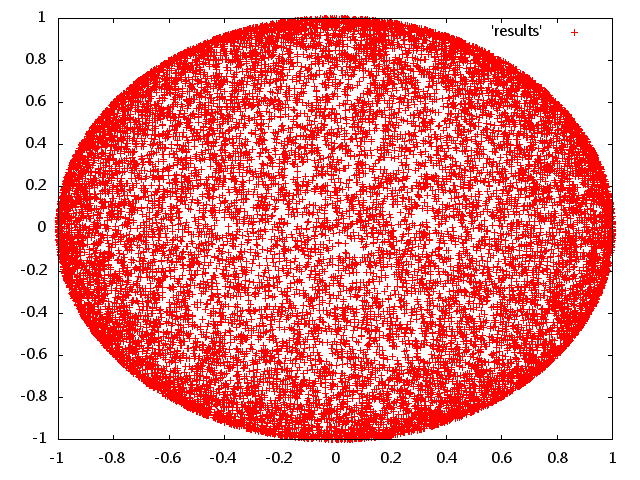
\includegraphics[width=3.5in]{sphere.png}
\end{center}
可以发现, 直观上看确实是球面上均匀分布的投影.

\section{验证 Marsaglia 抽样方法}
按照题目中给的算法编码, 主要代码为:
\begin{verbatim}
/* implements the marsaglia algorithm for sampling an uniform
   distribution over a sphere */
void rand_marsaglia(double *x, double *y)
{
    double u, v, r_squared;

start_all_over:
    u = rand_norm();
    v = rand_norm();
    r_squared = u*u + v*v;
    if (r_squared > 1)
        goto start_all_over;
    *x = 2*u * sqrt(1-r_squared);
    *y = 2*v * sqrt(1-r_squared);
}
\end{verbatim}
同上面一样生成数据点, 作出图形:
\begin{center}
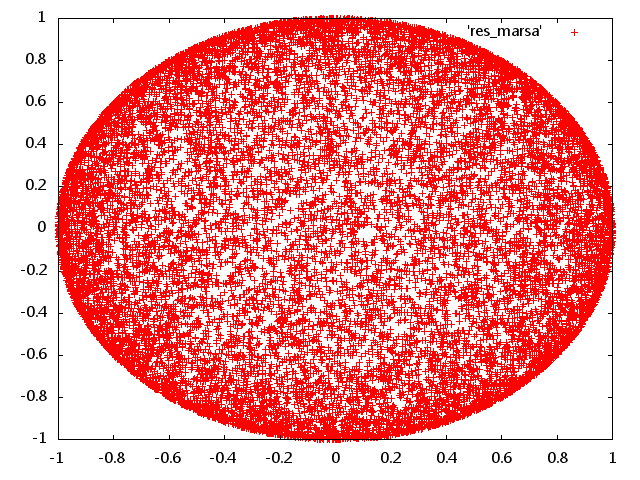
\includegraphics[width=3.5in]{sph_marsa.png}
\end{center}
发现和前面的结果几乎完全一样, 这样就验证了 Marsaglia 方法确实是有效的
从球面上均匀分布抽样的方法.

\end{document}